% 2008 年湖北卷文科第 19 题：矩形广告版式示意——左右两个大小相等的矩形栏目（阴影），
%   四周空白宽 10 cm，中缝空白宽 5 cm。
% 来源 PDF：gaokaomath-src/普通高考/2008/2008湖北文.pdf
% SHA-256：e097163e244cb8f03775ac7ff2e344ef85471e91ecc717d23698a0fb01e76963
% 原页：2008湖北文.pdf 第 2 页（A3 三栏）第 1 栏，书页码 452。
% 重绘依据：按原页画外框矩形，内部两个等宽阴影矩形，左右与上下留边等宽，两栏之间留中缝。
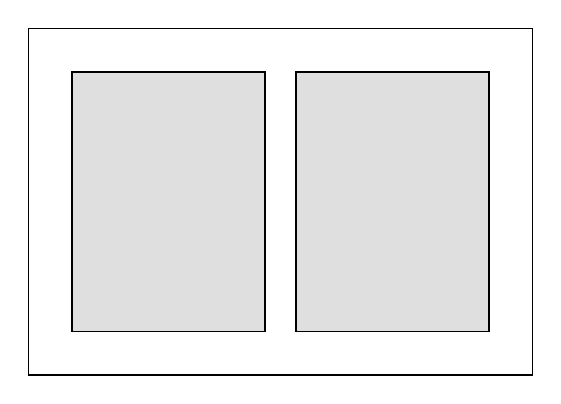
\begin{tikzpicture}[x=1.0cm, y=1.0cm, semithick]
  % 外框
  \draw (0,0) rectangle (6.4,4.4);
  % 两个栏目
  \fill[gray!25] (0.55,0.55) rectangle (3.00,3.85);
  \fill[gray!25] (3.40,0.55) rectangle (5.85,3.85);
  \draw (0.55,0.55) rectangle (3.00,3.85);
  \draw (3.40,0.55) rectangle (5.85,3.85);
\end{tikzpicture}
